\documentclass[12pt]{article}\usepackage[]{graphicx}\usepackage[]{color}
%% maxwidth is the original width if it is less than linewidth
%% otherwise use linewidth (to make sure the graphics do not exceed the margin)
\makeatletter
\def\maxwidth{ %
  \ifdim\Gin@nat@width>\linewidth
    \linewidth
  \else
    \Gin@nat@width
  \fi
}
\makeatother

\definecolor{fgcolor}{rgb}{0.345, 0.345, 0.345}
\newcommand{\hlnum}[1]{\textcolor[rgb]{0.686,0.059,0.569}{#1}}%
\newcommand{\hlstr}[1]{\textcolor[rgb]{0.192,0.494,0.8}{#1}}%
\newcommand{\hlcom}[1]{\textcolor[rgb]{0.678,0.584,0.686}{\textit{#1}}}%
\newcommand{\hlopt}[1]{\textcolor[rgb]{0,0,0}{#1}}%
\newcommand{\hlstd}[1]{\textcolor[rgb]{0.345,0.345,0.345}{#1}}%
\newcommand{\hlkwa}[1]{\textcolor[rgb]{0.161,0.373,0.58}{\textbf{#1}}}%
\newcommand{\hlkwb}[1]{\textcolor[rgb]{0.69,0.353,0.396}{#1}}%
\newcommand{\hlkwc}[1]{\textcolor[rgb]{0.333,0.667,0.333}{#1}}%
\newcommand{\hlkwd}[1]{\textcolor[rgb]{0.737,0.353,0.396}{\textbf{#1}}}%

\usepackage{framed}
\makeatletter
\newenvironment{kframe}{%
 \def\at@end@of@kframe{}%
 \ifinner\ifhmode%
  \def\at@end@of@kframe{\end{minipage}}%
  \begin{minipage}{\columnwidth}%
 \fi\fi%
 \def\FrameCommand##1{\hskip\@totalleftmargin \hskip-\fboxsep
 \colorbox{shadecolor}{##1}\hskip-\fboxsep
     % There is no \\@totalrightmargin, so:
     \hskip-\linewidth \hskip-\@totalleftmargin \hskip\columnwidth}%
 \MakeFramed {\advance\hsize-\width
   \@totalleftmargin\z@ \linewidth\hsize
   \@setminipage}}%
 {\par\unskip\endMakeFramed%
 \at@end@of@kframe}
\makeatother

\definecolor{shadecolor}{rgb}{.97, .97, .97}
\definecolor{messagecolor}{rgb}{0, 0, 0}
\definecolor{warningcolor}{rgb}{1, 0, 1}
\definecolor{errorcolor}{rgb}{1, 0, 0}
\newenvironment{knitrout}{}{} % an empty environment to be redefined in TeX

\usepackage{alltt}
%\VignetteDepends{devtools,knitr,spiders} 
%\VignetteEngine{knitr::knitr}
\usepackage{amsmath,amsfonts,amssymb,graphicx,
setspace,amsthm,subfig,authblk}
\usepackage [margin=1in]{geometry}
\usepackage{listings}
% \doublespacing
\usepackage{hyperref}
\hypersetup{pdfborder={0 0 0}, colorlinks=false, urlcolor=black}

\newcommand{\iid}{\stackrel{\mathrm{iid}}{\sim}}

\IfFileExists{upquote.sty}{\usepackage{upquote}}{}

\begin{document}
\title{Predator Preferences Model}
\author{S. Bonner and E. A. Roualdes}
\maketitle 



\section{Generic Model}
Strauss' statistic $L_{st}$ \cite{Strauss:1979} is the difference between $r_{st}$ the proportion of prey species $s$ found in the gut of a predator during occurrence $t$ and $p_{st}$ the proportion of prey species $s$ found in the habitat of said predator during occurrence $t$.  When the statistic $L_{st} := r_{st} - p_{st}$ is equal to zero we say the predator ate prey species $s$ randomly during time $t$.  A positive difference, $L_{st} > 0$, indicates preferential eating of prey species $s$, and negative values indicate aversion to prey species $s$ at time $t$.  We can replicate and add to the modeling considered by Strauss with the following set up.

Let $X_{jst} \sim \mathcal{P}(\lambda_{st})$ denote the number of prey species $s$ found in the gut of predator $j$ during occurrence $t$; $j \in \{1, \ldots, J\}, s \in \{1, \ldots, S\}, t \in \{1, \ldots, T\}$.  For now we ignore the fact that we only observe a $1$ if predator $j$ ate prey species $s$ during occurrence $t$ or a zero if the predator did not.  Further, $Y_{ist} \sim \mathcal{P}(\gamma_{st})$ will denote the number of prey species $s$ found in trap $i$, $i \in \{1, \ldots, I \}$, hypothesized to represent the habitat of predator $j$, during time occurrence $t$.  Interest lies in the null hypothesis

\begin{equation}
  \label{eq:null}
  H_0: \boldsymbol{\lambda}_t = c \boldsymbol{\gamma}_t, \forall t
\end{equation}

where $c \in \mathbb{R}$.  This hypothesis suggests that the predator's eating preferences are independent of time, i.e.\ the ratio of the rate at which the predator eats prey species $s$ to the rate at which prey species $s$ is found in the habitat is constant across time.  Strauss' $L$ is a special case of this framework where only a particular combination of prey species $s$ and time $t$ is considered, and $c$ is equal to the ratio of total number of prey found in the gut of the predator to the total number of prey found in the habitat.  

We first consider the parameters of this model under the null hypothesis.  Here, $S\cdot T + 1$ parameters will be estimated, $\gamma_{st}$ for $(s,t) \in \{S \times T\}$ and $c$. 

\begin{equation*}
  \hat{\gamma}_{st} = \frac{X_{\cdot st} + Y_{\cdot st}}{I\left(\frac{\sum_{st} X_{\cdot st}}{\sum_{st}Y_{\cdot st}} +1 \right)} \text{ and } \hat{c} = \frac{I\sum_{s,t} X_{\cdot st}}{J\sum_{s,t} Y_{\cdot st}}.
\end{equation*}

The parameters under the general alternative hypothesis,  $H_1:   \boldsymbol{\lambda}_t \ne c \boldsymbol{\gamma}_t, \forall t$, are simply the maximum likelihood estimates.

\begin{equation*}
  \hat{\lambda}_{st} = \frac{X_{\cdot st}}{J} \text{ and } \hat{\gamma}_{st} = \frac{Y_{\cdot st}}{I}
\end{equation*}

Null hypothesis (\ref{eq:null}) above is tested with the standard likelihood ratio statistic

\begin{equation}
  \label{eq:lrt}
  \Lambda(X,Y) := -2 \log{ \frac{ \sup L(\theta_0|X,Y)}{ \sup L(\theta_1|X,Y)} }
\end{equation}

where $\theta_0 = \{ \boldsymbol{\lambda}_t = c \boldsymbol{\gamma}_t, \forall t : (\gamma_{st}, c) \in \mathbb{R}^{ST+1} \}$ represents the likelihood under the null hypothesis, and $\theta_1 = \{ \boldsymbol{\lambda}_{st} \ne c \boldsymbol{\gamma}_{st} : (\lambda_{st}, \gamma_{st}) \in \mathbb{R}^{2ST} \}$ represents the likelihood under the alternative hypothesis.  Then $\Lambda \dot{\sim} \chi^2_{ST-1}$ and null hypothesis (\ref{eq:null}) is rejected when $P(\chi^2_{ST-1} > \Lambda) < \alpha$. 

\subsection{Unequal Trap Schedules}
Consider a situtation where the traps (catching prey species) were left out for a differing length of time within each occurrence, e.g.\ trap $i$ in month $t$ was left out for $6$ days, but trap $i'$ in month $t$ was left out for $3$ days.  We expect to catch an unequal number of prey in each trap simply because one trap was left out for a longer time within month $t$.  

Put $I_t := \sum_{i} numDays_{it}$ to be the total number of days all traps were left out during month $t$.  Then the complete data log-likelihood under this scenario is as follows.

\begin{equation*}
  l = -J\sum_{st}\lambda_{st} + \sum_{st}X_{\cdot st} \log{\lambda_{st}} - \sum_{t} I_t \sum_{s} \gamma_{st} + \sum_{st}Y_{\cdot st}\log{\gamma_{st}} + constant
\end{equation*}

If there exists a differing number of predators in each time period, we can similarly model this by indexing $J$ by $t$, say $J_t$.

\subsection{Non-Count Gut Data}

With smaller animals it is not always possible to observe a count of prey species eaten by a predator species.  Instead, a binary response of whether or not DNA of said prey species exists in the gut of the predator is observed.  In this case, we can treat the count of eaten prey species as missing and maximize the likelihood via the EM algorithm.  

We model what information we do observe.  Denote this binary response by $Z_{jst}$, which takes on the value $1$ if the $j^{th}$ predator ate prey species $s$ in time $t$ and $0$ otherwise.  Hence, $\Lambda(X,Y)$ is still calculable via the EM algorithm as follows.  Write out the complete data likelihood,

\begin{equation}
  \label{eq:llComp}
  L_{comp}(X,Z,Y|\boldsymbol{\lambda}, \boldsymbol{\gamma}) = \prod_{t}^T \prod_{s}^S \prod_{j}^J f_{X,Z}(x,z|\boldsymbol{\lambda})  f_{Y}(y|\boldsymbol{\gamma})
\end{equation}

\noindent Take the expectation of $\log{L_{comp}}$ with respect to the distribution of the missing data given the observed data and parameters, 


\begin{equation*}
  f_{X|Y,Z,\boldsymbol{\lambda},\boldsymbol{\gamma}}(x) = \frac{f_{X,Y,Z}(x,y,z|\boldsymbol{\gamma},\boldsymbol{\lambda})}{f_{Y,Z}(y,z|\boldsymbol{\lambda},\boldsymbol{\gamma})}. %= \frac{f_{X,Z}(x,z|\boldsymbol{\lambda})}{f_{Z}(z|\boldsymbol{\lambda})}.
\end{equation*}

\noindent Then maximize $\E_{X|Y,Z}l_{comp}$ with respect to the parameters $\gamma_{st}, \lambda_{st}, c$, just as above since here $X_{jst}$ is simply replaced by its expectation.

\section{Simulations}

In order to simulate and test data, we need to install an \texttt{R} package named \texttt{spiders}.  To install the package \texttt{spiders}, you can use \texttt{devtools}, or download the files from the \href{https://github.com/roualdes/spiders}{\texttt{GitHub}} webpage.

\begin{knitrout}
\definecolor{shadecolor}{rgb}{0.969, 0.969, 0.969}\color{fgcolor}\begin{kframe}
\begin{alltt}
\hlcom{## library(devtools) install_github('spiders',}
\hlcom{## 'roualdes')}
\hlkwd{library}\hlstd{(spiders)}
\end{alltt}
\end{kframe}
\end{knitrout}


We can then simulate some data by using the function \texttt{spiders::simData}.  Input to this function includes the number of predator species observed at each time point, the number of traps used at each time point, the number of prey species of interest, the number of time points for which measurements were taken, and rate parameters $\lambda_{st}, \gamma_{st}$ for which the predator ate and observed, respectively, prey species $s$ at time $t$.  For now, we assume that the number of predators and traps is fixed across time points.  Below we specify rate parameters that will be proportional across time; we expect to fail to reject null hypothesis (\ref{eq:null}) here. 

\begin{knitrout}
\definecolor{shadecolor}{rgb}{0.969, 0.969, 0.969}\color{fgcolor}\begin{kframe}
\begin{alltt}
\hlstd{Predators} \hlkwb{<-} \hlnum{77}
\hlstd{Traps} \hlkwb{<-} \hlnum{87}
\hlstd{PreySpecies} \hlkwb{<-} \hlnum{2}
\hlstd{Times} \hlkwb{<-} \hlnum{5}
\hlstd{ST} \hlkwb{<-} \hlstd{Times} \hlopt{*} \hlstd{PreySpecies}
\hlstd{l} \hlkwb{<-} \hlkwd{matrix}\hlstd{(}\hlnum{1}\hlstd{,} \hlkwc{nrow} \hlstd{= Times,} \hlkwc{ncol} \hlstd{= PreySpecies)}
\hlstd{g} \hlkwb{<-} \hlkwd{matrix}\hlstd{(}\hlnum{2}\hlstd{,} \hlkwc{nrow} \hlstd{= Times,} \hlkwc{ncol} \hlstd{= PreySpecies)}
\end{alltt}
\end{kframe}
\end{knitrout}


Simulate some data as follows.

\begin{knitrout}
\definecolor{shadecolor}{rgb}{0.969, 0.969, 0.969}\color{fgcolor}\begin{kframe}
\begin{alltt}
\hlstd{fdata} \hlkwb{<-} \hlkwd{simPref}\hlstd{(PreySpecies, Times, Predators, Traps, l,}
    \hlstd{g)}
\end{alltt}
\end{kframe}
\end{knitrout}


Then we can fit the model and calculate a p-value from these data.  The output of the model fit is below.

\begin{knitrout}
\definecolor{shadecolor}{rgb}{0.969, 0.969, 0.969}\color{fgcolor}\begin{kframe}
\begin{alltt}
\hlstd{(prefs} \hlkwb{<-} \hlkwd{predPref}\hlstd{(fdata}\hlopt{$}\hlstd{eaten, fdata}\hlopt{$}\hlstd{caught))}
\end{alltt}
\begin{verbatim}
$alt
$alt$gamma
  preySpecies1 preySpecies2
1        2.138        2.253
2        2.253        1.977
3        1.862        1.931
4        2.034        1.885
5        1.977        2.276

$alt$lambda
  preySpecies1 preySpecies2
1       1.0260       0.8831
2       1.0000       1.0260
3       0.9351       0.9740
4       1.1818       1.1169
5       1.0000       1.2208

$alt$SE
   lambda  gamma
11 0.1154 0.1568
21 0.1140 0.1609
31 0.1102 0.1463
41 0.1239 0.1529
51 0.1140 0.1507
12 0.1071 0.1609
22 0.1154 0.1507
32 0.1125 0.1490
42 0.1204 0.1472
52 0.1259 0.1617


$null
$null$gamma
  preySpecies1 preySpecies2
1        2.107        2.099
2        2.171        1.996
3        1.861        1.932
4        2.131        1.988
5        1.980        2.322

$null$c
[1] 0.5034

$null$SE
      c gamma11 gamma21 gamma31 gamma41 gamma51 
0.01782 0.12944 0.13138 0.12163 0.13017 0.12547 
gamma12 gamma22 gamma32 gamma42 gamma52 
0.12920 0.12597 0.12395 0.12572 0.13587 


$loglikH1
[1] 10206

$loglikH0
[1] 10202

$numPredators
[1] 77 77 77 77 77

$numTraps
[1] 87 87 87 87 87

$Lambda
[1] 7.293

$df
[1] 9

$p.value
[1] 0.6066

attr(,"class")
[1] "predPref"
\end{verbatim}
\end{kframe}
\end{knitrout}


An example where we reject the null hypothesis would have rate parameters that are differently proportional across time.  Consider the following.

\begin{knitrout}
\definecolor{shadecolor}{rgb}{0.969, 0.969, 0.969}\color{fgcolor}\begin{kframe}
\begin{alltt}
\hlstd{l} \hlkwb{<-} \hlkwd{matrix}\hlstd{(}\hlnum{1}\hlopt{:}\hlstd{ST,} \hlkwc{nrow} \hlstd{= Times,} \hlkwc{ncol} \hlstd{= PreySpecies)}
\hlstd{g} \hlkwb{<-} \hlkwd{matrix}\hlstd{(}\hlnum{2} \hlopt{*} \hlstd{(ST}\hlopt{:}\hlnum{1}\hlstd{),} \hlkwc{nrow} \hlstd{= Times,} \hlkwc{ncol} \hlstd{= PreySpecies)}
\hlstd{fdata} \hlkwb{<-} \hlkwd{simPref}\hlstd{(PreySpecies, Times, Predators, Traps, l,}
    \hlstd{g)}
\hlkwd{predPref}\hlstd{(fdata}\hlopt{$}\hlstd{eaten, fdata}\hlopt{$}\hlstd{caught)}\hlopt{$}\hlstd{p.value}
\end{alltt}
\begin{verbatim}
[1] 0
\end{verbatim}
\end{kframe}
\end{knitrout}


\subsection*{Tests}
\subsubsection*{Complete, Balanced Data}
We can test our functions by simulating many datasets with the same underlying parameters, fitting the model, and plotting the distribution of the estimates.  Let's first set the values of the parameters to be constant across time and species.

\begin{knitrout}
\definecolor{shadecolor}{rgb}{0.969, 0.969, 0.969}\color{fgcolor}\begin{kframe}
\begin{alltt}
\hlstd{l} \hlkwb{<-} \hlkwd{matrix}\hlstd{(}\hlnum{1.5}\hlstd{,} \hlkwc{nrow} \hlstd{= Times,} \hlkwc{ncol} \hlstd{= PreySpecies)}
\hlstd{g} \hlkwb{<-} \hlkwd{matrix}\hlstd{(}\hlnum{2} \hlopt{*} \hlstd{pi,} \hlkwc{nrow} \hlstd{= Times,} \hlkwc{ncol} \hlstd{= PreySpecies)}
\end{alltt}
\end{kframe}
\end{knitrout}


Using the function \texttt{spiders::testPref} we simulate $M=250$ datasets based on the above parameters and fit the model to each. By default, only $4$ of the $S*T = 10$ parameters of each $\boldsymbol{\lambda}$ and $\boldsymbol{\gamma}$ are stored.

\begin{knitrout}
\definecolor{shadecolor}{rgb}{0.969, 0.969, 0.969}\color{fgcolor}\begin{kframe}
\begin{alltt}
\hlstd{M} \hlkwb{<-} \hlnum{250}
\hlkwd{system.time}\hlstd{(out} \hlkwb{<-} \hlkwd{testPref}\hlstd{(PreySpecies, Times, Predators,}
    \hlstd{Traps, l, g,} \hlkwc{M} \hlstd{= M))}
\end{alltt}
\begin{verbatim}
   user  system elapsed 
  6.771   0.054   6.859 
\end{verbatim}
\end{kframe}
\end{knitrout}


Also output from this function is the number of iterations within \texttt{spiders::predPref}, in this case since we are fitting the complete, balanced data so there is only 

\begin{knitrout}
\definecolor{shadecolor}{rgb}{0.969, 0.969, 0.969}\color{fgcolor}\begin{kframe}
\begin{alltt}
\hlstd{out}\hlopt{$}\hlstd{iters[M, ]}
\end{alltt}
\begin{verbatim}
null gAtl 
   1    1 
\end{verbatim}
\end{kframe}
\end{knitrout}


for every simulated dataset.  

Since we know the value of the underlying parameters, we can plot these data and visually inspect our algorithm's performance using the function \texttt{spiders::plotTestPref}.

\begin{knitrout}
\definecolor{shadecolor}{rgb}{0.969, 0.969, 0.969}\color{fgcolor}\begin{kframe}
\begin{alltt}
\hlkwd{plotTestPref}\hlstd{(out}\hlopt{$}\hlstd{null, out}\hlopt{$}\hlstd{alt)}
\end{alltt}
\end{kframe}

{\centering \includegraphics[width=\maxwidth]{figure/unnamed-chunk-6} 

}



\end{knitrout}


To see that $c$ is estimated accurately, we use the fact that $\gamma_{st} = \gamma$ for all $\{s,t\}$ by averaging over the $4$ values of $\boldsymbol{\gamma}$ that were sampled: $\bar{\hat{c}}*\bar{\hat{\gamma}} = 1.5023$. 

Further, we can calculate and plot the estimated bias.  The boxplot contains the same randomly sampled parameters of $\lambda_{st},\gamma_{st}$ as before.  Here, the indices on the abcissa represent the enumeration of the set $\{(T,S)\}$ indexing $T$ first, e.g.\ index $8$ for would refer to the parameter value for the third time point of the second prey species since we have $5$ time points and $2$.   Averaged over all simulations, both mean (dot) and median (line), for each parameter value, are shown.

\begin{knitrout}
\definecolor{shadecolor}{rgb}{0.969, 0.969, 0.969}\color{fgcolor}\begin{kframe}
\begin{alltt}
\hlstd{bias} \hlkwb{<-} \hlkwd{calcBias}\hlstd{(out}\hlopt{$}\hlstd{null, out}\hlopt{$}\hlstd{alt, l, g)}
\hlkwd{plotBias}\hlstd{(bias)}
\end{alltt}
\end{kframe}

{\centering \includegraphics[width=\maxwidth]{figure/unnamed-chunk-7} 

}



\end{knitrout}


\subsubsection*{Complete, Unbalanced Data}

Here, we simply have to simulate an uneven number of predators and prey species caught in each time period. We do this and also create a more fun set of parameter values.

\begin{knitrout}
\definecolor{shadecolor}{rgb}{0.969, 0.969, 0.969}\color{fgcolor}\begin{kframe}
\begin{alltt}
\hlstd{Predators} \hlkwb{<-} \hlnum{4} \hlopt{*} \hlkwd{c}\hlstd{(}\hlnum{11}\hlstd{,} \hlnum{22}\hlstd{,} \hlnum{33}\hlstd{,} \hlnum{44}\hlstd{,} \hlnum{77}\hlstd{)}
\hlstd{Traps} \hlkwb{<-} \hlnum{3} \hlopt{*} \hlstd{Predators}\hlopt{/}\hlnum{4}
\hlstd{l} \hlkwb{<-} \hlkwd{matrix}\hlstd{(}\hlkwd{cbind}\hlstd{(}\hlnum{1}\hlopt{:}\hlnum{5}\hlstd{,} \hlnum{2}\hlopt{:}\hlnum{6}\hlstd{),} \hlkwc{nrow} \hlstd{= Times,} \hlkwc{ncol} \hlstd{= PreySpecies)}
\hlstd{g} \hlkwb{<-} \hlkwd{matrix}\hlstd{(pi,} \hlkwc{nrow} \hlstd{= Times,} \hlkwc{ncol} \hlstd{= PreySpecies)}
\end{alltt}
\end{kframe}
\end{knitrout}


Then we can simulate the data and plot it just as before.

\begin{knitrout}
\definecolor{shadecolor}{rgb}{0.969, 0.969, 0.969}\color{fgcolor}\begin{kframe}
\begin{alltt}
\hlkwd{system.time}\hlstd{(out} \hlkwb{<-} \hlkwd{testPref}\hlstd{(PreySpecies, Times, Predators,}
    \hlstd{Traps, l, g,} \hlkwc{M} \hlstd{= M))}
\end{alltt}
\begin{verbatim}
   user  system elapsed 
 15.807   0.072  16.225 
\end{verbatim}
\begin{alltt}
\hlkwd{plotTestPref}\hlstd{(out}\hlopt{$}\hlstd{null, out}\hlopt{$}\hlstd{alt)}
\end{alltt}
\end{kframe}

{\centering \includegraphics[width=\maxwidth]{figure/cu} 

}



\end{knitrout}


It is fairly obvious, by the bias plots, when the null hypothesis is false.

\begin{knitrout}
\definecolor{shadecolor}{rgb}{0.969, 0.969, 0.969}\color{fgcolor}\begin{kframe}
\begin{alltt}
\hlstd{bias} \hlkwb{<-} \hlkwd{calcBias}\hlstd{(out}\hlopt{$}\hlstd{null, out}\hlopt{$}\hlstd{alt, l, g)}
\hlkwd{plotBias}\hlstd{(bias)}
\end{alltt}
\end{kframe}

{\centering \includegraphics[width=\maxwidth]{figure/unnamed-chunk-9} 

}



\end{knitrout}


\subsubsection*{Non-Count Gut Data}
Similarly, we can test the EM algorithm using the same funciton, but declaring the variable \texttt{EM} to be true.

\begin{knitrout}
\definecolor{shadecolor}{rgb}{0.969, 0.969, 0.969}\color{fgcolor}\begin{kframe}
\begin{alltt}
\hlstd{Predators} \hlkwb{<-} \hlnum{124}
\hlstd{Traps} \hlkwb{<-} \hlnum{145}
\hlstd{l} \hlkwb{<-} \hlkwd{matrix}\hlstd{(}\hlnum{1.5}\hlstd{,} \hlkwc{nrow} \hlstd{= Times,} \hlkwc{ncol} \hlstd{= PreySpecies)}
\hlstd{g} \hlkwb{<-} \hlkwd{matrix}\hlstd{(}\hlnum{2} \hlopt{*} \hlstd{pi,} \hlkwc{nrow} \hlstd{= Times,} \hlkwc{ncol} \hlstd{= PreySpecies)}
\hlkwd{system.time}\hlstd{(out} \hlkwb{<-} \hlkwd{testPref}\hlstd{(PreySpecies, Times, Predators,}
    \hlstd{Traps, l, g,} \hlkwc{M} \hlstd{= M,} \hlkwc{EM} \hlstd{=} \hlnum{TRUE}\hlstd{))}
\end{alltt}
\begin{verbatim}
   user  system elapsed 
 51.223   0.127  51.494 
\end{verbatim}
\begin{alltt}
\hlkwd{plotTestPref}\hlstd{(out}\hlopt{$}\hlstd{null, out}\hlopt{$}\hlstd{alt)}
\end{alltt}
\end{kframe}

{\centering 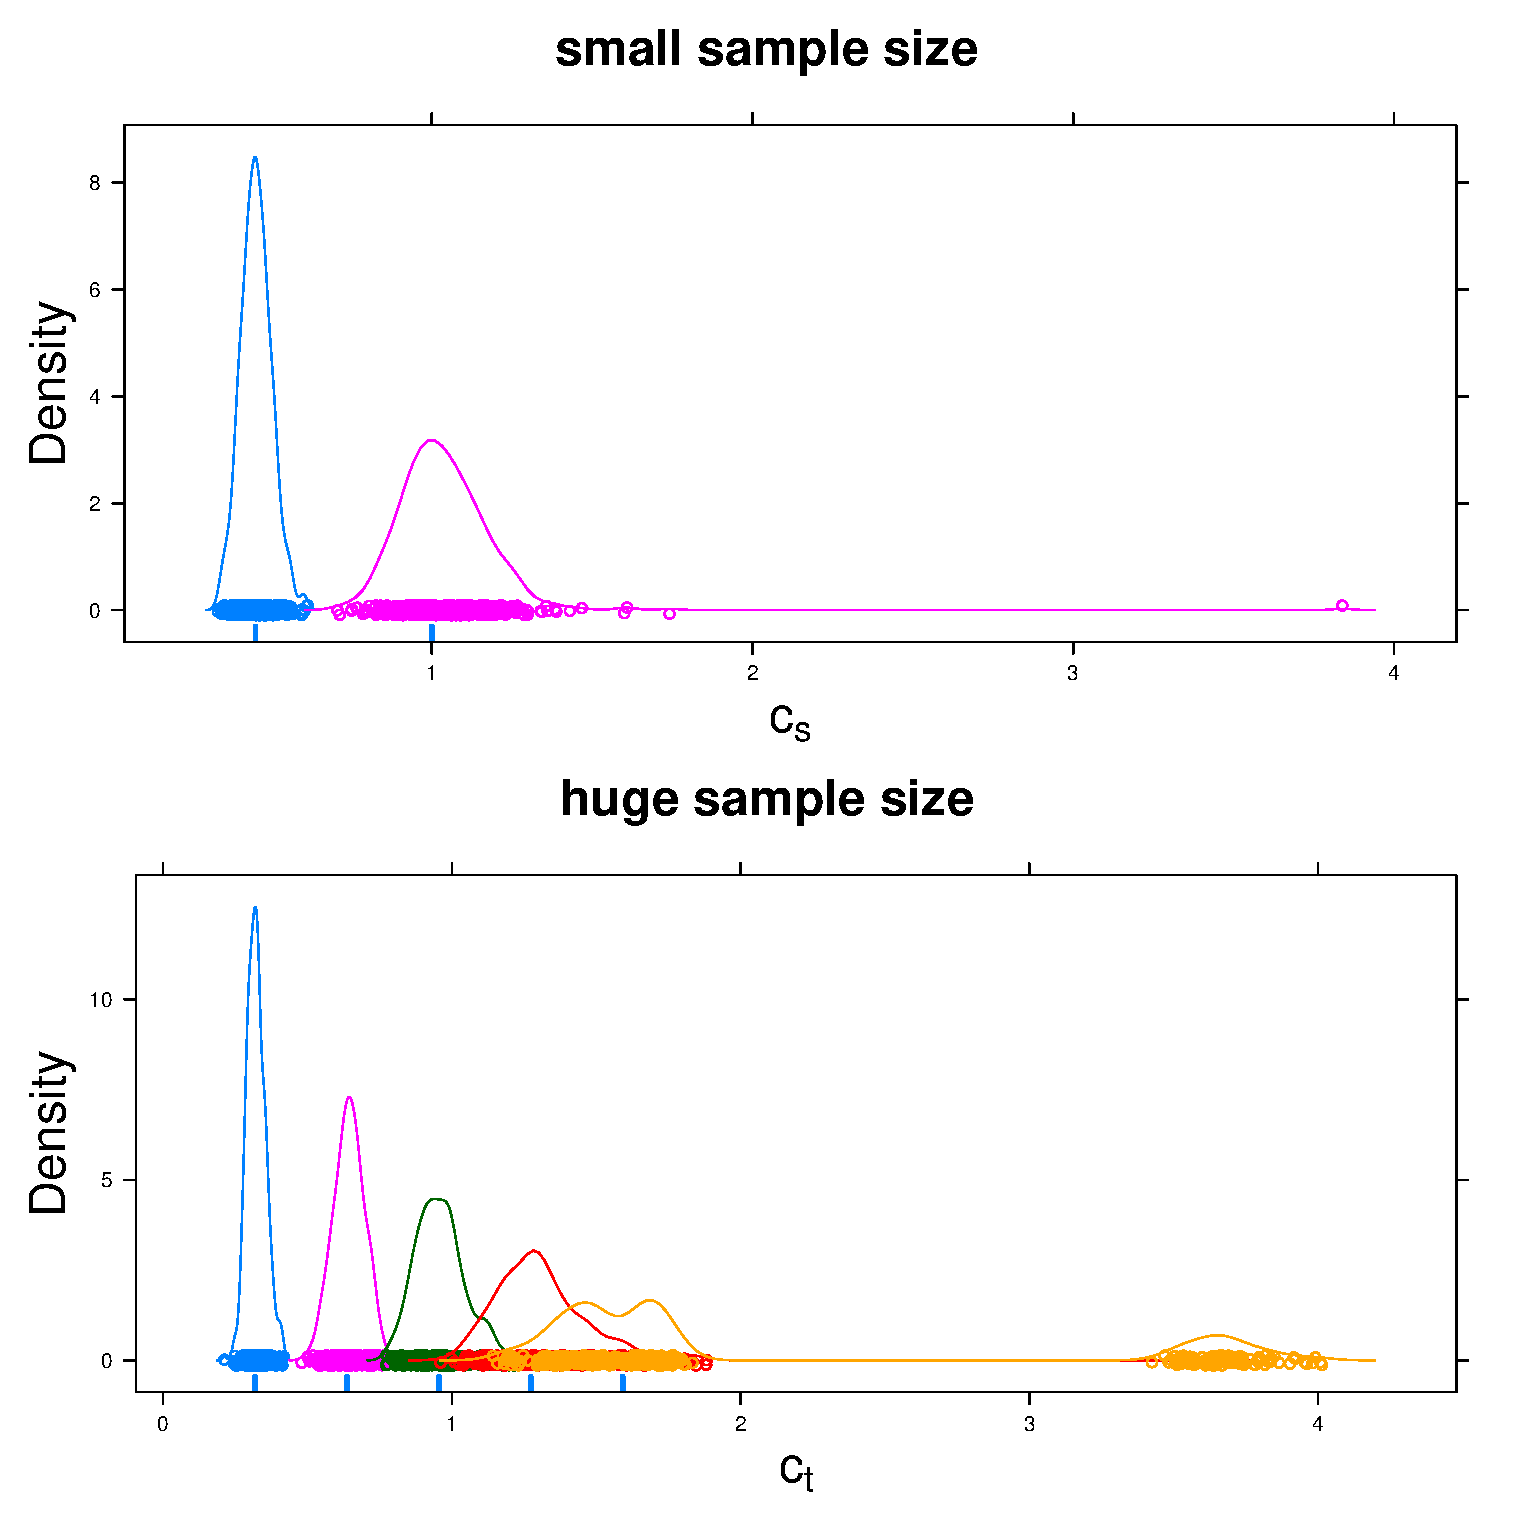
\includegraphics[width=\maxwidth]{figure/em} 

}



\end{knitrout}


The same as before, $c$ is estimated fairly well: $\bar{\hat{c}}*\bar{\hat{\gamma}} = 1.5055$.  Also, we can check how many iterations of the EM algorithm the last simulated dataset required

\begin{knitrout}
\definecolor{shadecolor}{rgb}{0.969, 0.969, 0.969}\color{fgcolor}\begin{kframe}
\begin{alltt}
\hlstd{out}\hlopt{$}\hlstd{iters[M, ]}
\end{alltt}
\begin{verbatim}
null gAtl 
  25   27 
\end{verbatim}
\end{kframe}
\end{knitrout}


\appendix
\section{Details}
\subsection{Complete, Balanced Data}
With balanced, count data the log-likelihood is

\begin{equation*}
  l = -J\sum_{s,t} \lambda_{st} + \sum_{s,t}X_{\cdot st}\log{\lambda_{st}} - I \sum_{s,t}\gamma_{st} + \sum_{s,t}Y_{\cdot st} + \text{const}.
\end{equation*}

Under $H_0: \lambda_{st} = c \gamma_{st}$ we find solutions of first derivatives of $l$ with respect to $c, \gamma_{st}$ set equal to zero to be

\begin{equation*}
  c = \frac{\sum_{s,t} X_{\cdot st}}{J\sum_{s,t} \gamma_{st}} \quad \text{ and } \quad \gamma_{st} = \frac{X_{\cdot st} + Y_{\cdot st}}{Jc + I}.
\end{equation*}

\noindent Solving these equations simultaneously gives

\begin{equation*}
  \hat{c} = \frac{J^{-1} \sum_{s,t} X_{\cdot st}}{I^{-1} \sum_{s,t} Y_{\cdot st}} \quad \text{ and } \quad \hat{\gamma}_{st} = \frac{X_{\cdot st} + Y_{\cdot st}}{I\left( \frac{\sum_{s,t}X_{\cdot st}}{\sum_{s,t} Y_{\cdot st}} + 1  \right)}.
\end{equation*}

Under $H_1: \lambda_{st} \ne \gamma_{st}$ we find the maximum likelihood estimates to be

\begin{equation*}
  \hat{\lambda}_{st} = \frac{X_{\cdot st}}{J} \quad \text{ and } \quad \hat{\gamma_{st}} = \frac{Y_{\cdot st}}{I}.
\end{equation*}

\subsection{Complete, Unbalanced Data}

With unbalanced, count data the log-likelihood is

\begin{equation*}
  l = -\sum_{t} J_t \sum_{s} \lambda_{st} + \sum_{s,t} X_{\cdot st} \log{J_t \lambda_{st}} - \sum_{t} I_t \sum_{s} \gamma_{st} + \sum_{s,t} Y_{\cdot st} \log{I_t \gamma_{st}}.
\end{equation*}

Under $H_0: \lambda_{st} = c \gamma_{st}$ we find solutions of first derivatives of $l$ with respect to $c, \gamma_{st}$ set equal to be

\begin{equation*}
  c = \frac{\sum_{s,t} X_{\cdot st}}{\sum_{t} J_t \sum_{s} \gamma_{st}} \quad \text{ and } \quad \gamma_{st} = \frac{X_{\cdot st} + Y_{\cdot st}}{cJ_{t} + I_{t}}.
\end{equation*}

\noindent Since we can't solve these equations simultaneously, we exploit the fact that the log-likelihood is concave; each term is concave and convexity is closed under addition.  Hence, we can iteratively maximize the profile log-likelihood until convergence.  

Under $H_1: \lambda_{st} \ne \gamma_{st}$ we find the maximum likelihood estimates to be

\begin{equation*}
  \hat{\lambda}_{st} = \frac{X_{\cdot st}}{J_{t}} \quad \text{ and } \quad \hat{\gamma}_{st} = \frac{Y_{\cdot st}}{I_{t}}.
\end{equation*}

\subsection{Non-Count Data}

When the count data are not observed we can fall back on treating the counts as missing, so long as we do observe indicators telling us when the predator species did eat prey species $s$.  

\subsubsection*{E-Step}
For this we need the conditional distribution of the missing data given the observed data

\begin{equation*}
  f_{X|Y,Z,\boldsymbol{\lambda},\boldsymbol{\gamma}}(x) =
    \frac{\exp{\{-\lambda_{st}\}} \lambda_{st}^{X_{jst}}}{(1 - \exp{\{-\lambda_{st}\}}) X_{jst}!} \quad \text{ where } \quad \E_{[X|Y,Z]}X_{jst} = \frac{\lambda_{st} \exp{\{\lambda_{st} \}}}{\exp{\{ \lambda_{st} \}} - 1}.
\end{equation*}

Since the joint density of $X_{jst}, Z_{jst}$ is

\begin{equation*}
  f_{X,Z|\boldsymbol{\lambda}}(x,z) = \left\{
    \begin{array}{lr}
      \exp{\{ -\lambda_{st} \}}, & X_{jst}=0 \mbox{ and } Z_{jst} = 0 \\
      \frac{\exp{\{-\lambda_{st} \}} \lambda_{st}^{X_{jst}}}{X_{jst}!}, & X_{jst} > 0 \mbox{ and } Z_{jst} = 1\\
      0 & \mbox{otherwise}
    \end{array}
  \right.
\end{equation*}

\noindent it is easy to calculate the expected value of the complete data log-likelihood

\begin{align*}
  \E l_{comp} 
  & = \E \log{f_{X,Z|\boldsymbol{\lambda}}(x,z)} + \log{f_{Y|\boldsymbol{\gamma}}(y)} \\
  & = \sum_{s=1}^S \sum_{t=1}^T \sum_{j=1}^{J_t} \E \log{f_{X,Z|\boldsymbol{\lambda}}(x_{jst},z_{jst})}
  + \sum_{s=1}^S \sum_{t=1}^T \sum_{i=1}^{I_t} \log{f_{Y|\boldsymbol{\gamma}}(y)} \\
  & = \sum_{s,t,j} \left( - \lambda_{st} 
    + z_{jst} \log(\lambda_{st}) \E X_{jst}  - \text{const} \right) - \sum_{s,t} \left( I_t \gamma_{st} + Y_{\cdot st} \log{I_t \gamma_{st}} \right).
\end{align*}

with respect to $f_{X|Y,Z,\boldsymbol{\lambda},\boldsymbol{\gamma}}$, where the expectation conditions on all of the remaining parameters.

%% \begin{equation*}
%%   \E l_{comp} = \sum_{s=1}^S \sum_{t=1}^T \sum_{j=1}^{J_t} \E[\log{f_{X,Z|\boldsymbol{\lambda}}(X_{jst},z_{jst})}]
%%   + \sum_{s=1}^S \sum_{t=1}^T \sum_{i=1}^{I_t} \log{f_{Y|\boldsymbol{\gamma}}(y)}
%% \end{equation*}
  
%% In this case we see
%% \begin{equation*}
%%   \log{f_{X,Z|\boldsymbol{\lambda}}(x_{jst},z_{jst})} =
%%   \left\{
%%     \begin{array}{ll}
%%       -\lambda_{st} & X_{jst} = 0 \mbox{ and } z_{jst}=0 \\
%%       -\lambda_{st} + X_{jst}\log(\lambda_{st})-\log(X_{st}!) & X_{jst} > 0 \mbox{ and } z_{jst}=1
%%     \end{array}
%%   \right.,
%% \end{equation*}

%% so that

%% \begin{equation*}
%%   \E[\log{f_{X,Z|\boldsymbol{\lambda}}(x_{jst},z_{jst})}] \equiv 
%%   - \lambda_{st} + z_{jst} \left[\frac{\lambda_{st}\exp(\lambda_{st})}{\exp(\lambda_{st})-1} \log(\lambda_{st})
%%     - \log(X_{st}!)\right].
%% \end{equation*}

%% Substituting this value back into the expected log-likelihood we then get:

\subsection*{M-Step}

We maximize $\E l_{comp}$ with respect to its parameters $\lambda_{st}, \gamma_{st}, c$, thus completing one step of the EM algorithm. 

\subsection*{Hypotheses Under EM}

Under $H_0: \lambda_{st} = c \gamma_{st}$, we iteratively solve the following equations within on step of the EM algorithm

\begin{equation*}
  \hat{\gamma}_{st} = \frac{z_{\cdot st} \E X_{jst} + Y_{\cdot st}}{cJ_t + I_t} \quad \text{ and } \quad \hat{c} = \frac{ \sum_{s,t} z_{\cdot st} \E X_{jst}}{\sum_{t} J_t \sum_{s} \gamma_{st}}.
\end{equation*}

Under $H_1$ we complete one step of the EM algorithm via

\begin{equation*}
  \hat{\lambda}_{st} = \frac{z_{\cdot st} \E X_{jst}}{J_t} \quad \text{ and } \quad \hat{\gamma}_{st} = \frac{Y_{\cdot st}}{I_t}.
\end{equation*}

\bibliographystyle{amsalpha}
\bibliography{refs}
\end{document}
